\documentclass[11pt,a4paper]{article}
\usepackage[a4paper,margin=1.45cm,top=1.1cm,bottom=1.1cm]{geometry}
\usepackage{fontspec}
\usepackage{graphicx,booktabs,amsmath,xcolor,enumitem,caption}
\usepackage[hidelinks]{hyperref}
\usepackage{titlesec}
\setmainfont{TeX Gyre Pagella}
\titleformat{\section}{\large\bfseries\color[HTML]{1F5C4A}}{\thesection}{0.6em}{}
\titlespacing*{\section}{0pt}{6pt}{2pt}
\captionsetup{font=small,labelfont=bf,skip=3pt}
\setlength{\parindent}{0pt}
\setlength{\parskip}{3pt}
\setlist{nosep,leftmargin=1.2em}
\pagestyle{empty}
\setlength{\intextsep}{4pt}\setlength{\textfloatsep}{5pt}\setlength{\floatsep}{4pt}

\begin{document}
\begin{center}
{\large\bfseries IE 643 Course Project: Novelty Assessment Report}\\[2pt]
{\bfseries Handwritten lecture notes to structured PDFs: diagnosing and fixing figure localisation}\\[2pt]
Team InTra \quad Ishaan Mane (25M1522) \quad Akshat Verma (25M1527)
\end{center}

\section{Problem and diagnosis}
\textbf{Pipeline.} The fine-tuned Qwen2.5-VL-7B~[1] (QLoRA~[2]) writes Markdown with one
\texttt{[Diagram: description]} line per drawing. Surya~[3] detects figure boxes, a renderer pairs each
description with a box, and Pandoc with XeLaTeX builds the PDF.
\begin{itemize}
\item \textbf{The problem.} Pairing used reading order only. It worked on slides (32 of 34 figures) but failed on
the dense IE802 notebook pages.
\item \textbf{Ground truth.} We drew a box for every drawing on the IE802 validation and test pages 041--056
(24 described drawings) and on 8 IE802 training pages kept for tuning only.
\item \textbf{Diagnosis.} A four-panel view per page shows the GT and Surya boxes, the \texttt{[Diagram]} lines
with their boxes, the placed crop and the PDF page. Each failure was assigned to one stage (Table~\ref{tab:diag}).
\item \textbf{Finding.} Matching caused most errors. Surya reads some pages in a different order than Qwen, a
drawing that Surya splits in two takes an extra slot and shifts every later pairing, and the merge rule glues
different drawings together. No figure was misplaced in the PDF.
\end{itemize}

\begin{table}[!h]\centering\small
\caption{Stage that decided each of the 24 placed IE802 figures under the old method (panel inspection).}\label{tab:diag}
\begin{tabular}{lccccc}\toprule
Outcome & correct & wrong: matching & partial: localisation & wrong: recognition & misplaced in PDF\\\midrule
Figures & 11 & 8 & 4 & 1 & 0\\\bottomrule
\end{tabular}
\end{table}
\vspace{-6pt}
{\small Two more drawings were never described by Qwen. The blind re-grade (Section 3) counts 13 correct
old crops, as it grades the crop a reader sees, not the failing stage.}

\section{Method: Surya decides where, Qwen decides which}
\begin{itemize}
\item \textbf{Grounding.} The base Qwen2.5-VL-7B (4-bit, LoRA adapter switched off) gives one rough bounding box
per description in its native grounding format. The box is loose, but it points at the right drawing.
\item \textbf{Pairing.} The Hungarian algorithm~[4] pairs descriptions with Surya boxes so that the total IoU
with the Qwen boxes is as large as possible, one box per description. Reading order no longer matters.
\item \textbf{Repair and fallback.} Surya pieces lying at least 60\% inside the same Qwen box are joined, which
repairs split drawings. If the result overlaps the Qwen box with IoU below $\tau=0.2$, the Qwen box is used.
$\tau$ was fixed on the training pages first. Arm C (ablation) uses the Qwen box alone.
\end{itemize}
\textbf{Three improvements}, each chosen on the training pages and then applied once:
\begin{enumerate}
\item \emph{Surya 2.5} instead of Surya 2. On all 410 pages figure precision rises from 0.73 to 0.83 (95\%
bootstrap interval of the gain +0.04 to +0.15), recall falls from 0.93 to 0.87, and it is 7\% faster.
\item \emph{Shared-box re-grounding.} When two descriptions get nearly the same Qwen box (IoU $\ge 0.7$), the
page is grounded again with one prompt that lists every description.
\item \emph{Completeness check.} The base Qwen scores ``is the whole sketch shown?'' for larger candidate crops
that contain the chosen box. A crop is enlarged only when the score rises by at least 0.05.
\end{enumerate}
Drawings with no description are recovered from leftover Surya boxes that Qwen calls a sketch (training pages:
5 of 9 recovered, 0 false).

\section{Evaluation and results}
\begin{itemize}
\item \textbf{Figure Error Score (FES).} A blind human re-grade. All 64 distinct crops of arms A, B and C were
shuffled with the method hidden and graded correct (0), loose or partial (0.5), or wrong or missing (1).
\item \textbf{Localisation Error (LE).} Automatic: $1-\mathrm{IoU}$ between the chosen box and the GT box.
\end{itemize}

\begin{table}[!h]\centering\small
\caption{IE802 validation and test pages. Left: blind grades of the three arms (24 descriptions). Right: each
improvement on the 23 descriptions that refer to a GT drawing.}\label{tab:res}
\begin{minipage}[t]{0.46\textwidth}\centering\footnotesize\setlength{\tabcolsep}{4pt}
\begin{tabular}{lccc}\toprule
Arm & FES $\downarrow$ & failed & mean LE $\downarrow$\\\midrule
A: reading order (old) & 0.42 & 9/24 & 0.58\\
\textbf{B: grounding + Hungarian} & \textbf{0.17} & \textbf{4/24} & 0.42\\
C: Qwen box only & 0.17 & 4/24 & 0.37\\\bottomrule
\end{tabular}
\end{minipage}\hfill
\begin{minipage}[t]{0.52\textwidth}\centering\footnotesize\setlength{\tabcolsep}{4pt}
\begin{tabular}{lccc}\toprule
Pipeline & right drawing & IoU $\ge$ 0.5 & mean LE $\downarrow$\\\midrule
B (Surya 2) & 21 & 14 & 0.42\\
+ Surya 2.5 & 21 & 16 & 0.39\\
+ shared-box re-grounding & \textbf{23} & 18 & 0.32\\
+ completeness check & \textbf{23} & \textbf{19} & \textbf{0.30}\\\bottomrule
\end{tabular}
\end{minipage}
\end{table}
\begin{figure}[!h]\centering
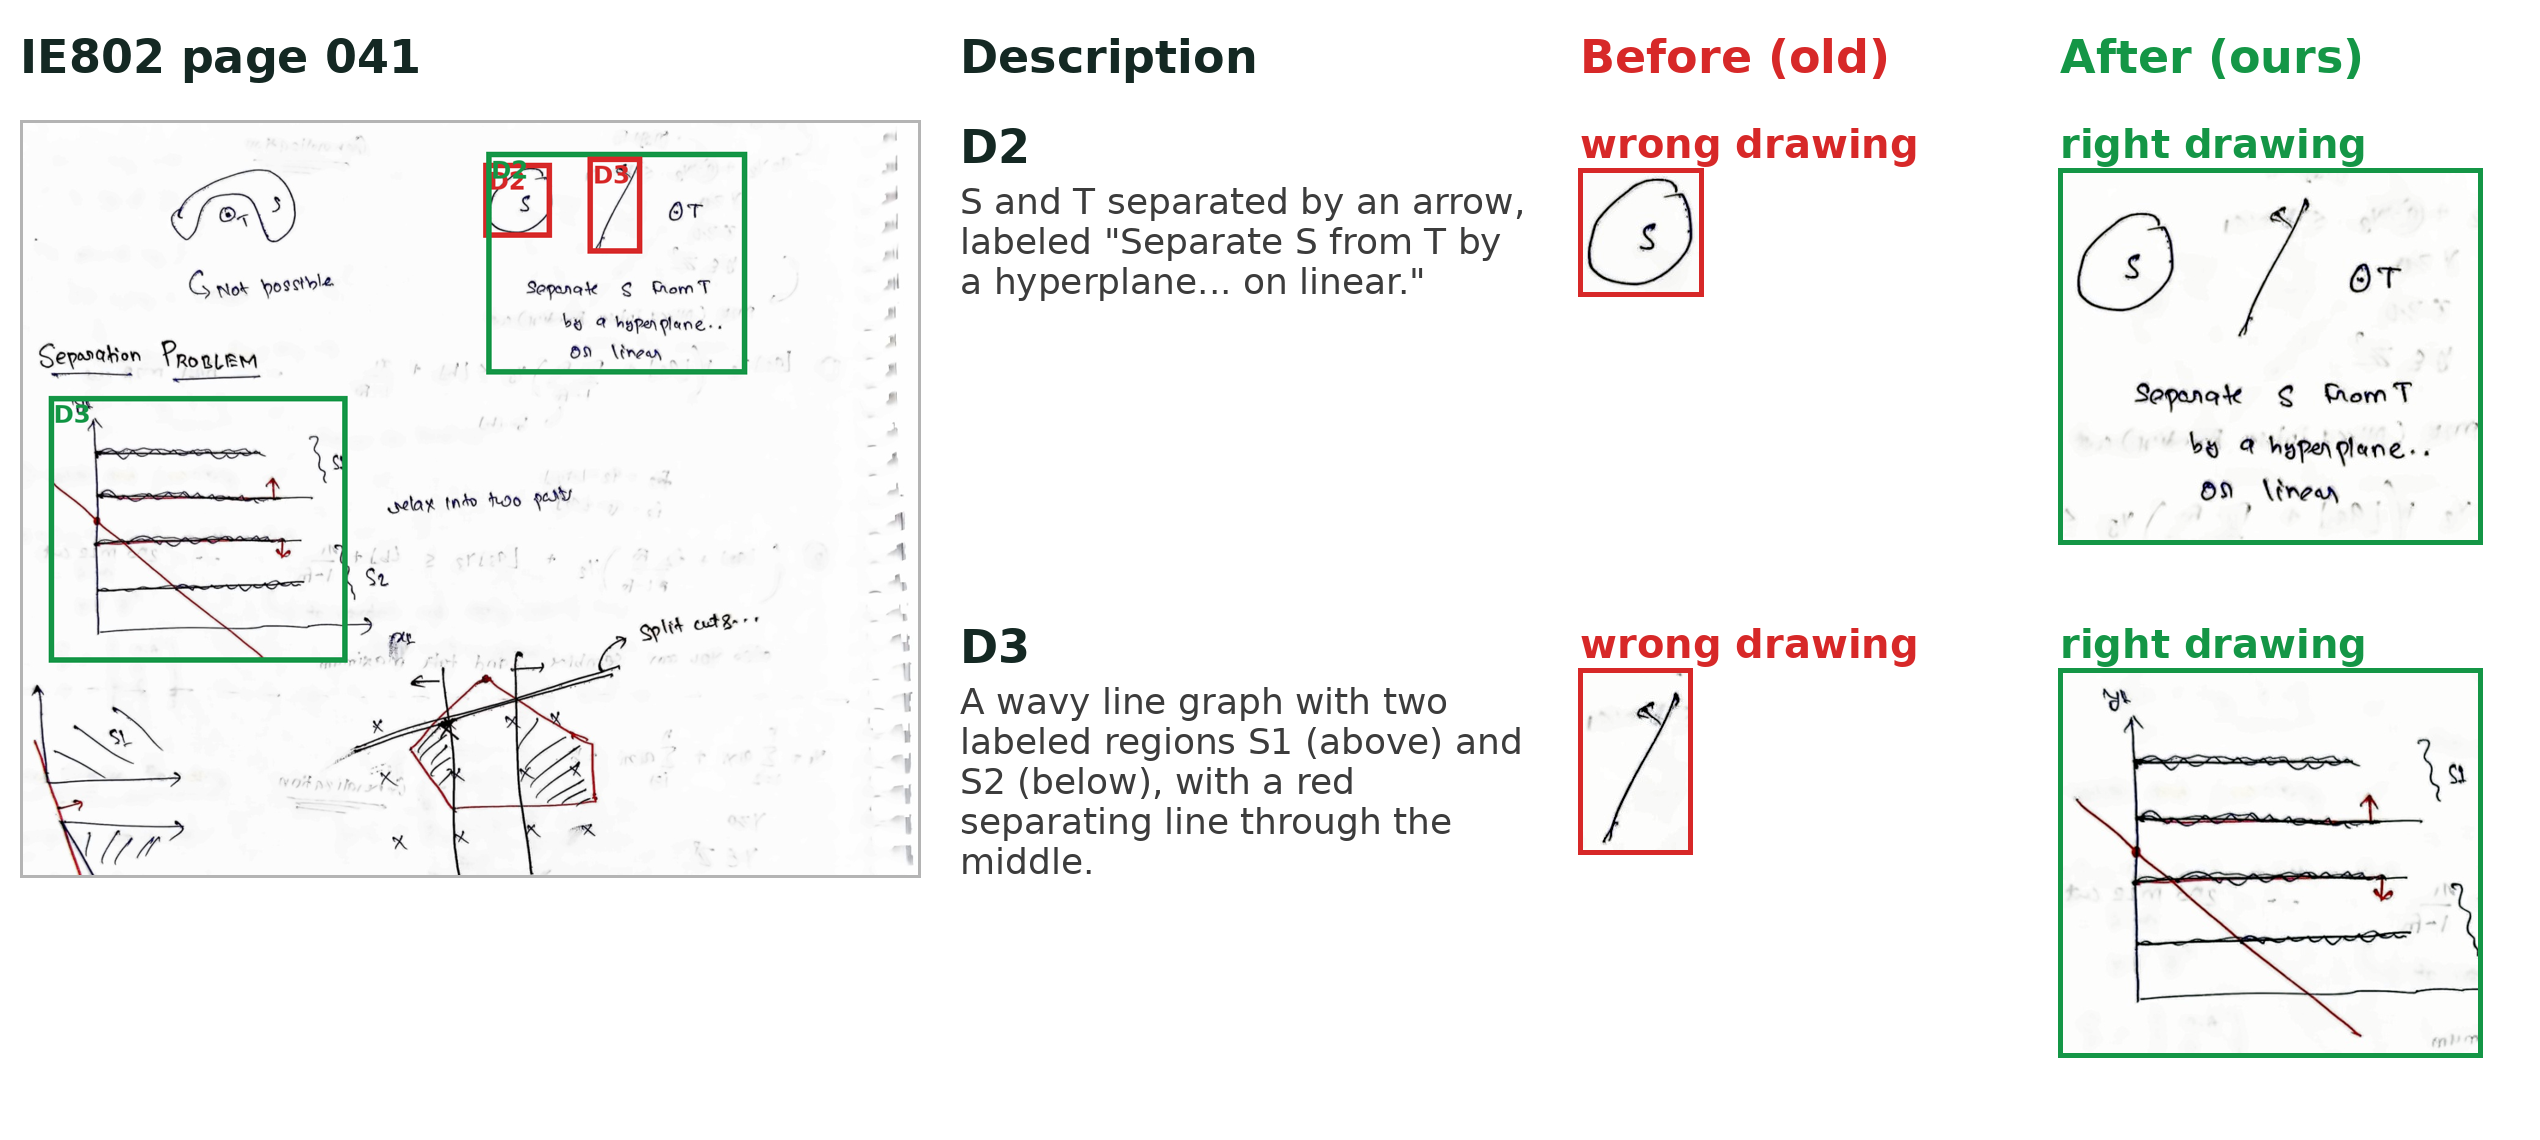
\includegraphics[width=0.5\textwidth]{page041_before_after.png}
\caption{IE802 page 041. Reading-order pairing put the wrong drawing under both captions (red). The final
pipeline places the right drawing, complete with its labels (green).}\label{fig:res}
\end{figure}
\vspace{-4pt}
\textbf{Key results}
\begin{itemize}
\item Method B halves the figure error (FES 0.42 to 0.17). It fixes eight IE802 descriptions and breaks one,
where Qwen gave two similar descriptions the same box. The shared-box re-grounding later repairs that case.
\item The final pipeline picks the right drawing for 23 of 23 descriptions and 19 of 23 boxes overlap the GT
with IoU $\ge 0.5$ (mean LE 0.58 to 0.30).
\item On the IE643 and MLT pages, 32 of 40 descriptions keep the identical crop and the 8 that change go from
1 to 6 correct.
\item Every later change was checked blind, side by side, on all crops it changed (AI grader, checked by the
team). Surya 2.5 beat Surya 2 in 10 of 20 pairs and lost 2 (sign test $p=0.039$). The completeness check won
3 of 7 and lost none.
\item A first verifier that could also pick \emph{smaller} crops looked better on LE (0.32 to 0.27) but lost
2 to 9 in the blind check, as tighter crops cut off labels. Overlap with GT alone can mislead.
\end{itemize}

\section{Self-verification and textbook footnotes}
\begin{itemize}
\item \textbf{Self-check.} The base Qwen sees each crop with its caption and answers whether it shows that
sketch. $P(\text{Yes})$ as a confidence score reaches an AUC of 0.82 on the 64 graded crops, and 5 of its 8
flags are real failures against a 23\% base rate. It spots the old method's swapped drawings ($P(\text{Yes})<0.04$) but catches only 1 of B's 5 failures
(4 on IE802, 1 on MLT), because B has already removed the errors it sees best.
\item \textbf{Footnotes.} For the IE643 test lectures, each section retrieves one passage from \emph{Dive into
Deep Learning}~[5] (CC BY-SA 4.0) with BM25~[6]. The base Qwen writes one or two sentences from that passage
only, citing its section, or answers NONE. Of 25 sections, 4 received NONE. Of the 21 footnotes, 18 are relevant and fully supported, 1 is
supported but only partly relevant, and 2 are unsupported, both after a wrongly retrieved passage.
\end{itemize}

\section{Maths, PDF quality and limitations}
\begin{itemize}
\item \textbf{Maths.} About 90\% of maths symbols are read correctly (symbol F1 0.895). Part of the remaining
error is our own labels writing one symbol two ways (\texttt{l} and \texttt{\textbackslash ell}). Scoring with
one notation lowers test NED from 0.311 to 0.302.
\item \textbf{Retrain.} One notation and larger input raised exact equation match from 0.17 to 0.23 but not
NED (0.302 vs 0.307, not significant), so the original model stays.
\item \textbf{PDF builder.} Headings now use one scale, with real lists and side captions, and every word is
kept. Pandoc dropped the YAML header (float pinning, \texttt{cancel}) when a header file was passed, which is
now fixed. The web demo runs the full new pipeline.
\item \textbf{Limitations.} 24 IE802 descriptions are a small test, so differences of one or two figures are
noise. Drawings that neither model finds stay missing. \textbf{Next steps:} consistent equation grouping in the labels, a detector trained on our GT boxes,
and TikZ redrawing of simple diagrams. Code: \url{https://github.com/aksh10-at/InTra-IE643}.
\end{itemize}

\vspace{2pt}
{\footnotesize\setlength{\parskip}{1pt}
\textbf{References}\\
{[1]} Shuai Bai, Keqin Chen, Xuejing Liu, Jialin Wang, Wenbin Ge, Sibo Song, Kai Dang, Peng Wang, Shijie Wang,
Jun Tang, Humen Zhong, Yuanzhi Zhu, Mingkun Yang, Zhaohai Li, Jianqiang Wan, Pengfei Wang, Wei Ding, Zheren Fu,
Yiheng Xu, Jiabo Ye, Xi Zhang, Tianbao Xie, Zesen Cheng, Hang Zhang, Zhibo Yang, Haiyang Xu and Junyang Lin.
Qwen2.5-VL Technical Report, arXiv, 2025. \url{https://arxiv.org/abs/2502.13923}\\
{[2]} Tim Dettmers, Artidoro Pagnoni, Ari Holtzman and Luke Zettlemoyer. QLoRA: Efficient Finetuning of
Quantized LLMs, NeurIPS, 2023. \url{https://arxiv.org/abs/2305.14314}\\
{[3]} Vik Paruchuri and Datalab. \url{https://github.com/datalab-to/surya}, Accessed on: 3rd October, 2026.\\
{[4]} Harold W. Kuhn. The Hungarian method for the assignment problem, Naval Research Logistics Quarterly, 1955.
\url{https://doi.org/10.1002/nav.3800020109}\\
{[5]} Aston Zhang, Zachary C. Lipton, Mu Li and Alexander J. Smola. Dive into Deep Learning, Cambridge
University Press, 2023. \url{https://d2l.ai}\\
{[6]} Stephen Robertson and Hugo Zaragoza. The Probabilistic Relevance Framework: BM25 and Beyond, Foundations
and Trends in Information Retrieval, 2009. \url{https://doi.org/10.1561/1500000019}
\par}
\end{document}
